\documentclass[14pt,a4paper]{report}  %紙張設定
\usepackage{xeCJK}%中文字體模組
%\setCJKmainfont{標楷體} %設定中文字體
\setCJKmainfont{MoeStandardKai.ttf}
%\newfontfamily\sectionef{Times New Roman}%設定英文字體
\newfontfamily\sectionef{Nimbus Roman}
\usepackage{enumerate}
\usepackage{amsmath,amssymb}%數學公式、符號
\usepackage{amsfonts} %數學簍空的英文字
\usepackage{graphicx, subfigure}%圖形
\usepackage{fontawesome5} %引用icon
\usepackage{type1cm} %調整字體絕對大小
\usepackage{textpos} %設定文字絕對位置
\usepackage[top=2.5truecm,bottom=2.5truecm,
left=3truecm,right=2.5truecm]{geometry}
\usepackage{titlesec} %目錄標題設定模組
\usepackage{titletoc} %目錄內容設定模組
\usepackage{textcomp} %表格設定模組
\usepackage{multirow} %合併行
%\usepackage{multicol} %合併欄
\usepackage{CJK} %中文模組
\usepackage{CJKnumb} %中文數字模組
\usepackage{wallpaper} %浮水印
\usepackage{listings} %引用程式碼
\usepackage{hyperref} %引用url連結
\usepackage{setspace}
\usepackage{lscape}%設定橫式
\lstset{language=Python, %設定語言
		basicstyle=\fontsize{14pt}{4pt}\selectfont, %設定程式內文字體大小
		frame=lines,	%設定程式框架為線
}
%\usepackage{subcaption}%副圖標
\graphicspath{{./../images/}} %圖片預設讀取路徑
\usepackage{indentfirst} %設定開頭縮排模組
\renewcommand{\figurename}{\Large 圖 } %更改圖片標題名稱
\renewcommand{\tablename}{\Large 表 }
\renewcommand{\lstlistingname}{\Large 程式 } %設定程式標示名稱
\hoffset=-5mm %調整左右邊界
\voffset=-8mm %調整上下邊界
\setlength{\parindent}{3em}%設定首行行距縮排
\usepackage{appendix} %附錄
\usepackage{diagbox}%引用表格
\usepackage{multirow}%表格置中
%\usepackage{number line}
%=------------------更改標題內容----------------------=%
\titleformat{\chapter}[hang]{\center\sectionef\fontsize{20pt}{1pt}\bfseries}{\LARGE 第\CJKnumber{\thechapter}章}{1em}{}[]
\titleformat{\section}[hang]{\sectionef\fontsize{18pt}{2.5pt}\bfseries}{{\thesection}}{0.5em}{}[]
\titleformat{\subsection}[hang]{\sectionef\fontsize{16pt}{2.5pt}\bfseries}{{\thesubsection}}{1em}{}[]
%=------------------更改目錄內容-----------------------=%
\titlecontents{chapter}[11mm]{}{\sectionef\fontsize{18pt}{2.5pt}\bfseries\makebox[3.5em][l]
{第\CJKnumber{\thecontentslabel}章}}{}{\titlerule*[0.7pc]{.}\contentspage}
\titlecontents{section}[18mm]{}{\sectionef\LARGE\makebox[1.5em][l]
{\thecontentslabel}}{}{\titlerule*[0.7pc]{.}\contentspage}
\titlecontents{subsection}[4em]{}{\sectionef\Large\makebox[2.5em][l]{{\thecontentslabel}}}{}{\titlerule*[0.7pc]{.}\contentspage}
%=----------------------章節間距----------------------=%
\titlespacing*{\chapter} {0pt}{0pt}{18pt}
\titlespacing*{\section} {0pt}{12pt}{6pt}
\titlespacing*{\subsection} {0pt}{6pt}{6pt}
%=----------------------標題-------------------------=%             
\begin{document} %文件
\sectionef %設定英文字體啟用
\vspace{12em}
\begin{titlepage}%開頭
\begin{center}   %標題  
\makebox[1.5\width][s]
{\fontsize{24pt}{2.5pt}國立虎尾科技大學}\\[18pt]
\makebox[1.2\width][s]
{\fontsize{24pt}{2.5pt}機械設計工程暨精密機械工程科}\\[18pt]
\makebox[1.5\width][s]
{\fontsize{24pt}{2.5pt}專題製作報告}\\[18pt]
%設定文字盒子 [方框寬度的1.5倍寬][對其方式為文字平均分分布於方框中]\\距離下方18pt
\vspace{6em} %下移
\fontsize{30pt}{1em}\selectfont\textbf
{
\vspace{0.5em}
有限元素法在四足機器人設計上的
應用}\\

\vspace{1em}
\sectionef\fontsize{30pt}{1em}\selectfont\textbf
{
\vspace{0.5em}
Application of Finite Element Method
\vspace{0.5em}
to
 \vspace{0.5em} 
Quadruped Robot Design}
 \vspace{1em}
%=---------------------參與人員-----------------------=%             
\end{center}
\begin{flushleft}
\begin{LARGE}

\hspace{32mm}\makebox[5cm][s]
{指導教授:\quad 嚴\quad 家\quad 銘\quad 老\quad 師}\\[6pt]
\hspace{32mm}\makebox[5cm][s]
{\phantom{指導教授:\quad}李\quad 武\quad 鉦\quad 老\quad 師}\\[6pt]

\hspace{32mm}\makebox[5cm][s]
{班\qquad 級:\quad 四\quad 設\quad 三\quad 乙}\\[6pt]
\hspace{32mm}\makebox[5cm][s]
{學\qquad 生:\quad 楊\quad 子\quad 頡\quad(40923231)}
\\[6pt]
\hspace{32mm}\makebox[5cm][s]
{\hspace{36.5mm}楊\quad 建\quad 霖\quad(40923233)}\\[6pt]
\hspace{32mm}\makebox[5cm][s]
{\hspace{36.5mm}詹\quad 侑\quad 儒\quad(40923235)}\\[6pt]
\hspace{32mm}\makebox[5cm][s]
{\hspace{36.5mm}蔡\quad 宗\quad 瑋\quad(40923240)}\\[6pt]
%設定文字盒子[寬度為5cm][對其方式為文字平均分分布於方框中]空白距離{36.5mm}\空白1em
\end{LARGE}
\end{flushleft}
\vspace{4em}
\fontsize{18pt}{2pt}\selectfont\hspace{1em}\centerline{\makebox[\width][s]
{中華民國\hspace{3em} 
\hspace*{-1em}一~一~二\quad 年\quad 六\quad 月}}
\end{titlepage}
\newpage
%=---------------專題製作合可證明---------------------=%
 {\renewcommand\baselinestretch{1.4}\selectfont %設定以下行距
 {\begin{center}
    {\fontsize{20pt}{2.5pt} {國立虎尾科技大學}\\[8pt]{機械設計工程暨精密機械工程科}\\[8pt]{學生專題製作合格認可證明}\\
    \hspace*{\fill} \\ %似enter鍵換行
    \par}
     \end{center}}
    {\begin{textblock}{60}(1.85,0.8)
    \noindent \fontsize{15pt}{16pt}\selectfont 專題製作修習學生\enspace:\quad
    {\begin{minipage}[t]{10em}\underline{四設三乙\enspace 40923231\enspace 楊子頡}\\ \underline{四設三乙\enspace 40923233\enspace 楊建霖}\\ \underline{四設三乙\enspace 40923235\enspace 詹侑儒}\\ \underline{四設三乙\enspace 40923240\enspace 蔡宗瑋}\\ %下劃線符號指令
    \end{minipage}}
         \par} %結束指定行距
    {\renewcommand\baselinestretch{1.2}\selectfont %設定以下行距
    {\begin{textblock}{30}(1.8,4)
    \noindent \fontsize{16pt}{16pt}\selectfont 專題製作題目\enspace :有限元素法在四足機器人設計上的應用
    \hspace*{\fill} \\
    \hspace*{\fill} \\
    \noindent \fontsize{16pt}{16pt}\selectfont 經評量合格,特此證明
    \hspace*{\fill} \\
    \hspace*{\fill} \\
    \noindent \fontsize{16pt}{16pt} \makebox[6em][s]{評審委員}\enspace:\quad
    {\begin{minipage}[t]{6em} \underline{            }\\[16pt] \underline{            }\\[16pt] \underline{            }\\
    \end{minipage}}
    \end{textblock}}
    {\begin{textblock}{10}(1.8,9)
    {\begin{flushleft}
    \fontsize{16pt}{16pt}\selectfont \makebox[6em][s]{指導老師}\enspace:\quad \underline{            }\\[10pt]
    \fontsize{16pt}{16pt}\selectfont \makebox[6em][s]{系主任}\enspace:\quad \underline{            }\\
    \hspace*{\fill} \\
    \fontsize{16pt}{2.5pt}\selectfont \makebox[12em][s]{中華民國~一一二年}\hspace{2pt}
    \fontsize{16pt}{2.5pt}\selectfont\makebox[8em][s]{六月七日}
    \end{flushleft}}
    \end{textblock}}
    \end{textblock}}
     \par} %結束指定行距
    \thispagestyle{empty}
     \newpage

%=------------------------摘要-----------------------=%
\renewcommand{\baselinestretch}{1.5} %設定行距
\pagenumbering{roman} %設定頁數為羅馬數字
\clearpage  %設定頁數開始編譯
\sectionef
\addcontentsline{toc}{chapter}{摘~~~要} %將摘要加入目錄
\begin{center}
\LARGE\textbf{摘~~~要}\\
\end{center}

\begin{flushleft}
\raggedright
\fontsize{14pt}{20pt}\sectionef\hspace{12pt}\quad 本研究旨在探討如何利用ODOO PLM進行協同設計,以提高團隊合作效率和品質。通過分析ODOO PLM在協同設計過程中的應用效果,並提出相關的優化建議,以改善設計流程並推動協同設計的應用。\\[14pt]

\fontsize{14pt}{20pt}\sectionef\hspace{12pt}\quad 以鋼球平衡台設計為例,我們將透過ODOO PLM和GitHub進行協同設計、管理、製造執行及整合功能。設計過程中,我們將使用Geogebra、Onshape和Solidworks等工具設計機構,並透過CoppeliaSim和Python進行PID控制模擬。同時,使用自行維護的3D列印機製作所需零件,以實現虛實整合之目標。最後根據ODOO PLM和GitHub的記錄歷程,評估協同作業的工作模式。\\[12pt]

\end{flushleft}



\vspace{6cm}


\begin{hangparas}{1.5cm}{1}
關鍵字:比例-積分-微分控制器 (PID)、產品生命週期管理 (PLM)、協同 (CD)、CoppeliaSim、Github
\end{hangparas}


\newpage

%=--------------------Abstract----------------------=%
\renewcommand{\baselinestretch}{1.5} %設定行距
\addcontentsline{toc}{chapter}{Abstract} %將摘要加入目錄
\begin{center}
\LARGE\textbf\sectionef{Abstract}\\
\begin{flushleft}
\fontsize{14pt}{16pt}\sectionef\hspace{12pt}\quad This study aims to explore the utilization of ODOO PLM for collaborative design to enhance team cooperation efficiency and quality. By analyzing the application effectiveness of ODOO PLM in collaborative design processes and proposing relevant optimization suggestions, the research seeks to improve design workflows and promote the application of collaborative design.\\[12pt]

\fontsize{14pt}{16pt}\sectionef\hspace{12pt}\quad Using the design of a steel ball balancing platform as an example, collaborative design, management, manufacturing execution, and integration functionalities will be conducted through ODOO PLM and GitHub. Throughout the design process, tools such as Geogebra, Onshape, and Solidworks will be employed to design mechanisms, with CoppeliaSim and Python utilized for PID control simulation. Additionally, required components will be fabricated using a self-maintained 3D printer to achieve the goal of virtual and real integration. Finally, based on the record history of ODOO PLM and GitHub, the collaborative operation mode will be evaluated.\\
\end{flushleft}


\vspace{3cm}
% \fontsize{14pt}{16pt}\selectfont\sectionef Keywords: proportional–integral–derivative controller (PID), Product Lifecycle Management (PLM),collaborative(CD), CoppeliaSim ,Github
\begin{hangparas}{1.5cm}{1}
Keywords: proportional–integral–derivative controller (PID), Product Lifecycle Management (PLM),collaborative(CD), CoppeliaSim ,Github
\end{hangparas}




\newpage
%=------------------------謝辭----------------------=%
\addcontentsline{toc}{chapter}{誌~~~謝}
\centerline\LARGE\textbf{誌~~謝}\\
\begin{flushleft}
\fontsize{14pt}{2.5pt}\hspace{12pt}\quad 本專題能完成有著許多人員的幫忙,大四學長他們不吝嗇地將往年的製作經驗傳授給我們,讓我們在製作的時候少走了許多錯路,還總是貼心找出重點提醒我們可以加以描述。再來是我們的指導教授嚴家銘教授,他提供了多方面的資訊,拋出問題並給予建議,擬定了我們小組有限元素法研究和學習方向,開會也時常提出建議以及未來發展,得以順利解決遇到的技術問題,同時也給了相當程度的自由,讓小組得以有彈性去尋探索及摸索,而本專題組員也充分地付出了許多,讓專題研究能順利完成,從中獲益良多,特此感謝。
\end{flushleft}
\newpage
%=------------------------目錄----------------------=%
\renewcommand{\contentsname}{\centerline{\fontsize{18pt}{\baselineskip}\selectfont\textbf{目\quad 錄}}}
\tableofcontents  %目錄產生
\newpage
%=------------------圖表目錄產生----------------------=%
\renewcommand{\listfigurename}{\centerline{\fontsize{18pt}{\baselineskip}\selectfont\textbf{圖\quad 目\quad 錄 }}}
\newcommand{\loflabel}{圖} %定義\loflabel 文字為圖
\renewcommand{\numberline}[1]{\loflabel~\fontsize{14pt}{12pt}\selectfont #1\hspace*{0.5em}}
\listoffigures

\newpage

\renewcommand{\listtablename}{\centerline{\fontsize{18pt}{\baselineskip}\selectfont\textbf{表\quad 目\quad 錄 }}}
\newcommand{\lotlabel}{表} %定義\lotlabel 文字為表
\renewcommand{\numberline}[1]{\lotlabel~\fontsize{14pt}{12pt}\selectfont #1\hspace*{0.5em}}
\listoftables
%----------------------------------------%

\end{center}
%=-------------------------內容----------------------=%
\chapter{前言}
\renewcommand{\baselinestretch}{10.0} %設定行距
\pagenumbering{arabic} %設定頁號阿拉伯數字
\setcounter{page}{1}  %設定頁數
\fontsize{14pt}{2.5pt}\sectionef
\section{設計架構}
此次 pj3 專題目標有建立場景中的計時器、球員外型及移動優化、添加球員擊球和翻車再起能、進球後收集並隨機投下新的一顆球、建立以機械式轉盤傳動計分系統。由於目標繁多,需要組員間分工負責,在每個禮拜的協同中逐步完成 pj3 專題。\\

\begin{figure}[hbt!]
\begin{center}
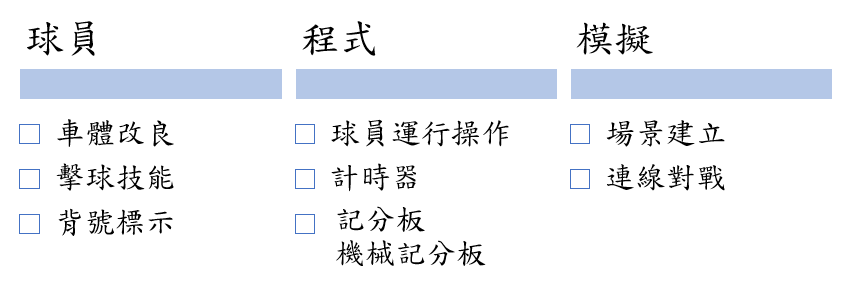
\includegraphics[width=15cm]{35}
\caption{\Large 設計目標圖}\label{fig.35}
\end{center}
\end{figure}
\section{規則說明}\emph{}
類似於足球遊戲,一開始時球會置於場中央,遊戲開始後雙方即可以鍵盤操控機器人,透過防守敵方以及與隊友間的傳球推球至已方的球門得分。\\
遊戲規則如下:
\begin{enumerate}
\item 球觸碰到球門感測器即算得分。
\item 在十分鐘的比賽時間內,獲得最多分數的隊伍即獲勝。
\item 任一方進球得分後,隨機在場內投下新的球,雙方接續進行比賽。
\end{enumerate}

\renewcommand{\baselinestretch}{0.5} %設定行距

%=---------------------參考文獻----------------------=%
\addcontentsline{toc}{chapter}{參考文獻} % 新增目錄名稱
\newpage
\renewcommand\bibname{參~考~文~獻}
\begin{thebibliography}{99}  % 參考文獻印出之編號最寬為兩個字母寬

\bibitem{item1} ALEXANDER HASP FRANK. MORGAN TJERNSTRÖM. 2019. 
\bibitem{item2} \href{https://www.odoo.com/documentation/16.0/zh_TW/applications/inventory_and_mrp/plm.html}
\bibitem{item3} \href{https://link.springer.com/book/10.1007/978-3-030-98578-3}
\bibitem{item4} \href{https://link.springer.com/book/10.1007/978-3-031-50658-1}
\bibitem{item5} \href{https://link.springer.com/book/10.1007/978-3-319-75804-6}
\bibitem{item6} \href{https://zhuanlan.zhihu.com/p/382346258}
\bibitem{item7} N. Apazidis, Mekanik II, Partikelsystem, stel kropp och analytisk mekanik, vol. 1:3. Studentlitteratur AB, 2017.
\bibitem{item8} \href{https://mde.tw/pj40922/content/index.html}

\end{thebibliography}
\newpage

%=---------------附錄-----------------=%
\addcontentsline{toc}{chapter}{附錄} %新增目錄名稱
\begin{appendix}
\renewcommand{\thesection}{\bf 附錄 \Alph{section}}%設定標題名稱
\begin{center}
\fontsize{20pt}{0em}\selectfont\bf 附錄
\end{center}
\section*{LaTeX}
LaTex 為一種程式語言,支援標準庫 (Standard Libraries) 和外部程式庫 (External Libraries),不過與一般程式語言不同的是,它可以直接表述 Tex 排版結構,類似於 PHP 之於 HTML 的概念。但是直接撰寫 LaTex 仍較複雜,因此可以藉由 Markdown 這種輕量的標註式語言先行完成文章,再交由 LaTex 排版。
此專題報告採用編輯軟體為LaTeX,綜合對比Word編輯方法,LaTeX較為精準正確、更改、製作公式等,以便符合規範、製作。
 \begin{table}[htbp] %htbp代表表格浮動位置
			\centering%表格居中
			\caption{文字編輯軟體比較表}%表:標題
			\large%字體大小
			\label{tab_文字編輯軟體比較表:scale}
			\begin{tabular}{|c|c|c|c|c|c|c|}
			\hline
			\diagbox[width=5em]& 相容性 & 直觀性 & 文件排版 & 數學公式 & 微調細部\\ 
			\hline
			LaTeX 		&$\surd$&		&$\surd$&$\surd$&$\surd$\\
			\hline
			Word	 	&		&$\surd$&		&		&$\surd$\\
			\hline
			
			\end{tabular}
		\end{table}	
\end{appendix}
\begin{itemize} 
\item 特點:
\end{itemize}
\begin{enumerate}
\item 相容性:以Word為例會有版本差異,使用較高版本編輯的文件可能無法以較低的版本開啟,且不同作業系統也有些許差異;相比LaTeX可以利用不同編譯器進行編譯,且為免費軟體也可移植至可攜系統內,可以搭配Github協同編譯。
\item 文件排版:許多規範都會要求使用特定版型,使用文字編譯環境較能準確符合規定之版型,且能夠大範圍的自定義排定所需格式,並能不受之後更改而整體格式變形。
\item 數學公式呈現:LaTex可以直接利用本身多元的模組套件加入、編輯數學公式,在數學推導過程能夠快速的輸入自己需要的內容即可。
\item 細部調整:在大型論文、報告中有多項文字、圖片、表格,需要調整細部時,要在好幾頁中找尋,而LaTeX可以分段章節進行編譯,再進行合併處理大章節。
\end{enumerate}
\newpage

\section*{足端軌跡}
利用GeoGebra軟體求得各種足端軌跡所需的轉軸角度。\

\begin{figure}[htbp]
  \centering
  \begin{minipage}{0.45\linewidth}
    \centering
    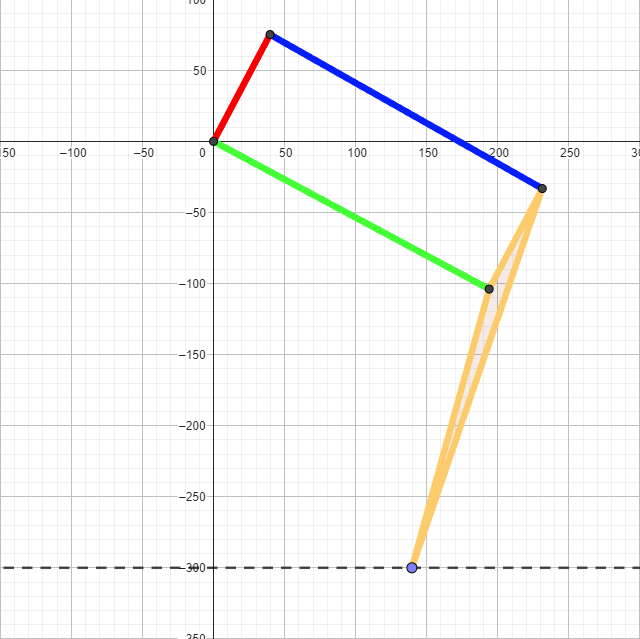
\includegraphics[height=5cm,width=5cm]{足端軌跡(直線)}
    \caption{足端軌跡(直線)}
    \label{足端軌跡(直線)}
  \end{minipage}
  \hfill
  \begin{minipage}{0.45\linewidth}
    \centering
    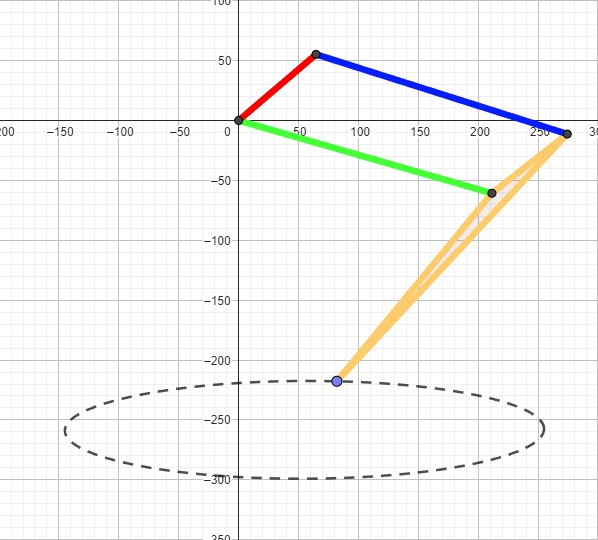
\includegraphics[height=5cm,width=5cm]{足端軌跡(橢圓)}
    \caption{足端軌跡(橢圓)}
    \label{足端軌跡(橢圓)}
  \end{minipage}
  
  \vspace{0.2cm} % 調整垂直間距
  
  \begin{minipage}{0.45\linewidth}
    \centering
    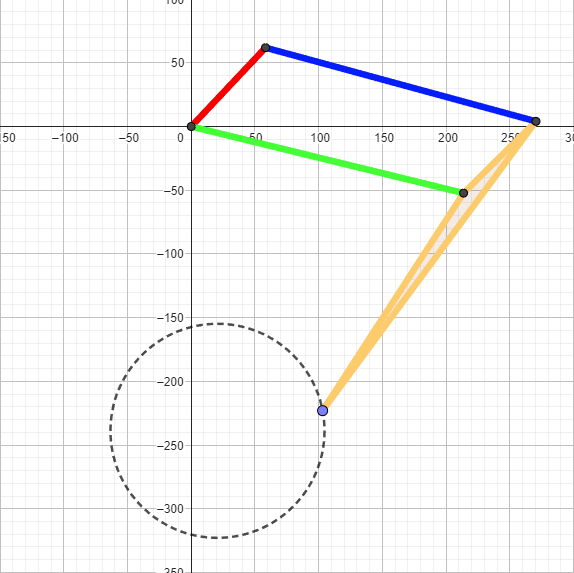
\includegraphics[height=5cm,width=5cm]{足端軌跡(圓形)}
    \caption{足端軌跡(圓形)}
    \label{足端軌跡(圓形)}
  \end{minipage}
  \hfill
  \begin{minipage}{0.45\textwidth}
    \centering
    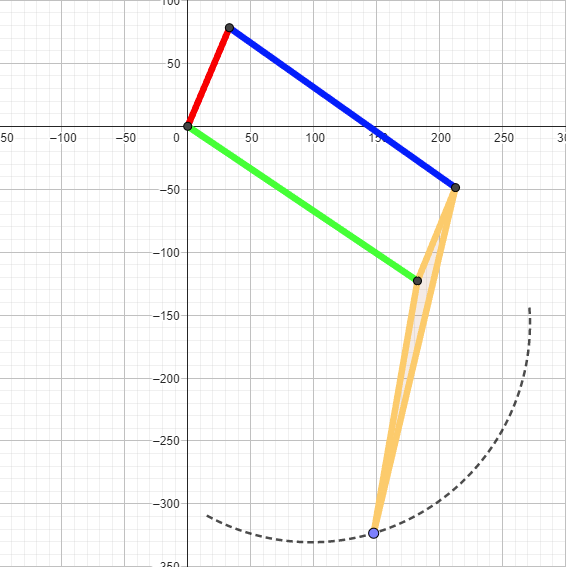
\includegraphics[height=5cm,width=5cm]{足端軌跡(弧線)}
    \caption{足端軌跡(弧線)}
    \label{足端軌跡(弧線)}
  \end{minipage}
  
  \vspace{0.2cm} % 調整垂直間距
  
  \begin{minipage}{0.45\linewidth}
    \centering
    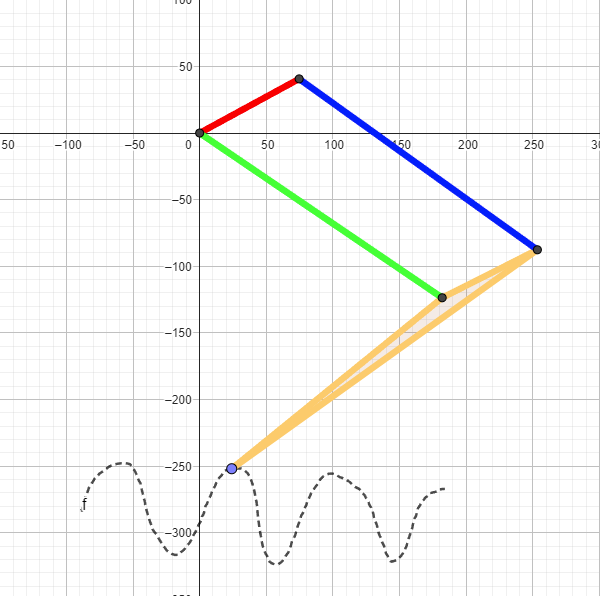
\includegraphics[height=5cm,width=5cm]{足端軌跡(不規則)}
    \caption{足端軌跡(不規則)}
    \label{足端軌跡(不規則)}
  \end{minipage}
\end{figure}
  
\newpage

\newpage
%=-------------作者簡介-----------------=%
    \addcontentsline{toc}{chapter}{作者簡介}
    \begin{center}
	\fontsize{20pt}{0em}\selectfont \bf{作者簡介}\\
	\end{center}	
	{\begin{textblock}{6}(0,0.5)
	\begin{figure}
	
\includegraphics[width=1.25in]{41023218}
	\end{figure}
	\end{textblock}}
	{\renewcommand\baselinestretch{0.99}\selectfont %設定以下行距
	{\begin{textblock}{15}(3.5,0.7)%{寬度}(以左上角為原點之右移量,下移量)
	\noindent\fontsize{14pt}{0em}\selectfont \makebox[4em][s]{姓名}\enspace:\enspace
    \fontsize{14pt}{0em}\selectfont \makebox[4em][s]{楊子頡}\\     \hspace*{\fill} \\
    \fontsize{14pt}{0em}\selectfont \makebox[4em][s]{學號}\enspace:\enspace
    \fontsize{14pt}{0em}\selectfont \makebox[4em][s]{40923231} \\ %\makebox為文本盒子
    \hspace*{\fill} \\
    \fontsize{14pt}{0em}\selectfont \makebox[4em][s]{就讀學校}\enspace:\enspace
    \fontsize{14pt}{0em}\selectfont \makebox[9em][s]{國立虎尾科技大學~機械設計工程系}\\
    \hspace*{\fill} \\
    \fontsize{14pt}{0em}\selectfont \makebox[4em][s]{經歷}\enspace:\enspace
    \fontsize{14pt}{0em}\selectfont \makebox[9em][s]{國立彰化師範大學附屬高級工業職業學校}\\
    \fontsize{14pt}{0em}\selectfont \makebox[4em][s]{\quad}\enspace\enspace
    \fontsize{14pt}{0em}\selectfont \makebox[8em][s]{機電科}\\
    \end{textblock}}}
   % \hspace*{\fill} \\
   \vspace{2em}
	{\begin{textblock}{6}(0,2.3)
	\begin{figure}
	
\includegraphics[width=1.15in]{41023248} 
    \end{figure}
    \end{textblock}}
    {\renewcommand\baselinestretch{0.99}
    \selectfont %設定以下行距
    {\begin{textblock}{15}(3.5,2.5) %{寬度}(以左上角為原點之右移量,下移量)
\noindent\fontsize{14pt}{0em}\selectfont \makebox[4em][s]{姓名}\enspace:\enspace
\fontsize{14pt}{0em}\selectfont \makebox[4em][s]{楊建霖}\\ 
\hspace*{\fill} \\
\fontsize{14pt}{0em}\selectfont \makebox[4em][s]{學號}\enspace:\enspace
\noindent\fontsize{14pt}{0em}\selectfont \makebox[4em][s]{40923233} \\ 
\hspace*{\fill} \\
\fontsize{14pt}{0em}\selectfont \makebox[4em][s]{就讀學校}\enspace:\enspace
\fontsize{14pt}{0em}\selectfont \makebox[9em][s]{國立虎尾科技大學~機械設計工程系}\\
\hspace*{\fill} \\
\fontsize{14pt}{0em}\selectfont \makebox[4em][s]{經歷}\enspace:\enspace
\fontsize{14pt}{0em}\selectfont \makebox[9em][s]{國立秀水高級工業職業學校}\\
\fontsize{14pt}{0em}\selectfont \makebox[4em][s]{\quad}\enspace\enspace
\fontsize{14pt}{0em}\selectfont \makebox[8em][s]{製圖科}\\
    \end{textblock}}}
    %\hspace*{\fill} \\
    \vspace{2em}
    {\begin{textblock}{6}(0,4.1)
    \begin{figure}
        
\includegraphics[width=1.15in]{41023251} %{}內是圖片文件的相對路徑
    \end{figure}
    \end{textblock}}
    {\renewcommand\baselinestretch{0.99}\selectfont %設定以下行距
    {\begin{textblock}{15}(3.5,4.3) %{寬度}(以左上角為原點之右移量,下移量)
\noindent\fontsize{14pt}{0em}\selectfont \makebox[4em][s]{姓名}\enspace:\enspace%\noindent指定首行不進行縮排
\fontsize{14pt}{0em}\selectfont \makebox[4em][s]{詹侑儒}\\ 
\hspace*{\fill} \\
\noindent\fontsize{14pt}{0em}\selectfont \makebox[4em][s]{學號}\enspace:\enspace
\noindent\fontsize{14pt}{0em}\selectfont \makebox[4em][s]{40923235} \\ %\makebox為文本盒子
\hspace*{\fill} \\
\noindent\fontsize{14pt}{0em}\selectfont \makebox[4em][s]{就讀學校}\enspace:\enspace
\noindent\fontsize{14pt}{0em}\selectfont \makebox[9em][s]{國立虎尾科技大學~機械設計工程系}\\
\hspace*{\fill} \\
\noindent\fontsize{14pt}{0em}\selectfont \makebox[4em][s]{經歷}\enspace:\enspace
\fontsize{14pt}{0em}\selectfont \makebox[9em][s]{新北市立新莊高級中學}\\
    \end{textblock}}}
   % \hspace*{\fill} \\
   \vspace{2em}
    {\begin{textblock}{6}(0,5.9)
    \begin{figure}
        
\includegraphics[width=1.15in]{41023254} %{}內是圖片文件的相對路徑
    \end{figure}
    \end{textblock}}
    {\renewcommand\baselinestretch{0.99}\selectfont %設定以下行距
    {\begin{textblock}{15}(3.5,6.1) %{寬度}(以左上角為原點之右移量,下移量)
\noindent\noindent\fontsize{14pt}{0em}\selectfont \makebox[4em][s]{姓名}\enspace:\enspace
\noindent\fontsize{14pt}{0em}\selectfont \makebox[4em][s]{蔡宗瑋}\\ \hspace*{\fill} \\
\noindent\fontsize{14pt}{0em}\selectfont \makebox[4em][s]{學號}\enspace:\enspace
\noindent\fontsize{14pt}{0em}\selectfont \makebox[4em][s]{40923240} \\ \hspace*{\fill} \\
\noindent\fontsize{14pt}{0em}\selectfont \makebox[4em][s]{就讀學校}\enspace:\enspace
\noindent\fontsize{14pt}{0em}\selectfont \makebox[9em][s]{國立虎尾科技大學~機械設計工程系}\\
\hspace*{\fill} \\
\noindent\fontsize{14pt}{0em}\selectfont \makebox[4em][s]{經歷}\enspace:\enspace
\fontsize{14pt}{0em}\selectfont \makebox[9em][s]{國立秀水高級工業職業學校}\\
\fontsize{14pt}{0em}\selectfont \makebox[4em][s]{\quad}\enspace\enspace
\fontsize{14pt}{0em}\selectfont \makebox[8em][s]{製圖科}\\
    \end{textblock}}}
\newpage

%=----------------書背----------------------=%
\pagestyle{empty}%設定沒有頁眉和頁腳
\begin{center}
\fontsize{0.001pt}{1pt}\selectfont .\\
\vspace{2em}
\fontsize{30pt}{30pt}\selectfont 【05】 \\
\fontsize{20pt}{20pt}\selectfont
\vspace{0.1em}
分\\
類\\
編\\
號\\
\vspace{0.1em}
\hspace{-0.5em}:\\
\vspace{0.1em}
\rotatebox[origin=cc]{270}{\sectionef\LARGE \textbf{112-4-CAE-3006、3004-1}}\\ %旋轉
\vspace{0.1em}
有\\
限\\
元\\
素\\
法\\
在\\
四\\
足\\
機\\
器\\
人\\
上\\
的\\
應\\
用\\
\vspace{1em}
一\\
\vspace{0.1em}
百\\
\vspace{0.1em}
一\\
\vspace{0.1em}
十\\
\vspace{0.1em}
三\\
\vspace{0.1em}
級\\

\end{center}
%\newpage
%\begin{landscape}  %橫式環境
%\begin{center}
%\fontsize{0.001pt}{1pt}\selectfont .
%\vspace{70mm}
%\rotatebox[origin=cc]{90}{\LARGE 【14】}\rotatebox[origin=cc]%{180}{\LARGE 1-2-APP-8765} %旋轉
%\end{center}
%\end{landscape}
\end{document}
